\documentclass[12pt,a4paper]{article}
\usepackage[utf8]{inputenc}
\usepackage[T1]{fontenc}
\usepackage{lmodern}
\usepackage[a4paper,margin=1in]{geometry}
\usepackage{amsmath,amssymb}
\usepackage{hyperref}
\usepackage{booktabs}
\usepackage{graphicx}
\usepackage{listings}
\usepackage{xcolor}
\usepackage{enumitem}
\usepackage{caption}
\usepackage{chngcntr}
\usepackage{float}
\usepackage{needspace}
\usepackage{tabularx}
\usepackage{tikz}
\usetikzlibrary{calc}

\hypersetup{
  colorlinks=true,
  linkcolor=blue!50!black,
  urlcolor=blue!50!black,
  pdftitle={Dua Technical Report: Sistem Linear Banded dan Pemodelan Lintasan Bintang},
  pdfauthor={}
}

\lstdefinestyle{pseudo}{
  basicstyle=\ttfamily\small,
  frame=single,
  breaklines=true,
  columns=fullflexible,
  keepspaces=true,
  showstringspaces=false,
  captionpos=b
}

\setlength{\parindent}{0pt}
\setlength{\parskip}{0.45em}
\renewcommand{\arraystretch}{1.12}
\renewcommand{\contentsname}{Daftar Isi}
\renewcommand{\lstlistingname}{Kode}
\counterwithin{table}{section}
\AtBeginDocument{\counterwithin{lstlisting}{section}}

\title{Dua Technical Report: Sistem Linear Banded dan Pemodelan Lintasan Bintang}
\author{}
\date{}

\begin{document}
\begin{titlepage}
\thispagestyle{empty}
\centering

\vspace*{0.45cm}
{\Large\bfseries Tugas Kelompok 1\par}
\vspace{0.08cm}
{\Large\bfseries Technical Report\par}
{\large Analisis Numerik B\par}

\vspace{0.7cm}
\includegraphics[width=0.31\textwidth]{cover_assets/ui_logo_crop_v2.png}\par

\vspace{0.55cm}
{\large\bfseries Anggota:\par}
\vspace{0.2cm}
{\small
Farras Hafizhudin Indra Wijaya (2106652682)\par
Haekal Alexander Dinova (2406352424)\par
Anderson Tirza Liman (2406355893)\par
Jovanus Irwan Susanto (2406434140)\par
}

\vspace{0.55cm}
\fcolorbox{blue!70!black}{blue!70!black}{
\parbox{0.88\textwidth}{\centering\color{white}\bfseries Pakta Integritas}
}

\noindent
\fcolorbox{blue!70!black}{blue!3}{
\parbox{0.88\textwidth}{
\raggedright Dengan ini, kami menyatakan bahwa tugas ini adalah hasil pekerjaan kelompok kami sendiri.\par
\raggedleft Kelompok B3
}
}

\vspace{0.4cm}
\renewcommand{\arraystretch}{1.08}
\footnotesize
\begin{tabular}{|>{\centering\arraybackslash}p{0.20\textwidth}|>{\centering\arraybackslash}p{0.20\textwidth}|>{\centering\arraybackslash}p{0.20\textwidth}|>{\centering\arraybackslash}p{0.20\textwidth}|}
\hline
\parbox[c][3.1cm][c]{0.185\textwidth}{\centering \includegraphics[height=0.95cm]{cover_assets/signature_farras_final.png}\\[0.08cm]Farras\\Hafizhudin\\Indra Wijaya} &
\parbox[c][3.1cm][c]{0.185\textwidth}{\centering \includegraphics[height=0.95cm]{cover_assets/signature_dinova_black_v3.png}\\[0.08cm]Haekal\\Alexander\\Dinova} &
\parbox[c][3.1cm][c]{0.185\textwidth}{\centering \includegraphics[height=0.95cm]{cover_assets/signature_anderson_final.png}\\[0.08cm]Anderson\\Tirza Liman} &
\parbox[c][3.1cm][c]{0.185\textwidth}{\centering \includegraphics[height=0.95cm]{cover_assets/signature_jovanus_final.png}\\[0.08cm]Jovanus\\Irwan\\Susanto} \\
\hline
\end{tabular}

\end{titlepage}

\clearpage
\tableofcontents
\clearpage

\section*{Technical Report I: Block LU dan Thomas Algorithm untuk Sistem Linear Banded}
\addcontentsline{toc}{section}{Technical Report I: Block LU dan Thomas Algorithm untuk Sistem Linear Banded}

\subsection*{Rangkuman}
Laporan pertama membahas implementasi dan evaluasi dua pendekatan untuk menyelesaikan sistem persamaan linear banded, yaitu \textbf{Block LU Factorization} dan \textbf{Thomas algorithm}. Dari identifikasi struktur matriks input, diperoleh bahwa data asli mempunyai lower bandwidth $p=1$ dan upper bandwidth $q=2$, sehingga matriks memang berada pada kelas \emph{banded system}. Fakta ini penting karena pada kelas banded, pilihan algoritma seharusnya tidak lagi dipandang sebagai satu solusi tunggal untuk semua kasus, melainkan disesuaikan dengan struktur pita yang tersedia.

Dalam kerangka ini, Block LU dipakai sebagai metode \emph{general-purpose} untuk \emph{banded system} yang belum cukup spesial untuk ditangani oleh solver compact seperti Thomas atau variasinya. Implementasi yang dipakai pada laporan ini tetap menyimpan matriks kerja dalam bentuk dense, tetapi organisasi blocked-nya menjaga locality komputasi lebih baik daripada LU non-blocked. Kebijakan backend yang dipakai adalah: untuk ukuran $n<512$, perhitungan dilakukan di CPU, sedangkan untuk $n\geq512$, operasi \emph{triangular solve} dan Schur complement dipindahkan ke GPU. Sebaliknya, Thomas algorithm dipakai untuk kasus tridiagonal, yaitu subkelas banded yang memang mempunyai struktur cukup spesifik untuk dieksploitasi langsung dengan array satu dimensi.

Hasil eksperimen menunjukkan bahwa pada matriks tridiagonal sintetis berukuran sampai $512$, Thomas algorithm selalu lebih cepat daripada Block LU. Sebagai contoh, pada ukuran $512$, Block LU membutuhkan sekitar $21.5605$ ms, sedangkan Thomas algorithm hanya sekitar $5.3477$ ms. Analisis kompleksitas mendukung temuan ini: Block LU tetap memiliki biaya waktu orde $O(n^3)$ dan memori orde $O(n^2)$, sedangkan Thomas algorithm hanya membutuhkan waktu dan memori orde $O(n)$. Dari sisi akurasi, error Thomas algorithm tetap sangat kecil dan stabil pada seluruh ukuran yang diuji.

Kesimpulan utamanya adalah bahwa pemilihan algoritma harus mengikuti struktur matriks. Untuk \emph{banded system} yang tidak mempunyai struktur cukup spesial untuk solver khusus, Block LU masih merupakan pendekatan umum yang masuk akal. Namun untuk \emph{banded system} spesial seperti matriks tridiagonal, algoritma yang sadar struktur seperti Thomas jauh lebih efisien tanpa mengorbankan akurasi.

\section{Pendahuluan}
Tujuan utama studi ini adalah membandingkan dua pendekatan penyelesaian sistem linear banded, yaitu Block LU dan Thomas algorithm, dengan memperhatikan tiga aspek utama: efisiensi penyimpanan, biaya komputasi, dan akurasi solusi. Motivasi studi ini muncul dari fakta bahwa matriks input sering kali mempunyai struktur pita yang bisa dikenali lebih awal. Bila struktur tersebut diketahui sejak awal, maka baik struktur data maupun algoritma penyelesaiannya seharusnya dapat dipilih secara lebih tepat.

Dalam laporan ini, pembahasan dimulai dari identifikasi karakteristik matriks dan konsekuensinya terhadap penyimpanan. Setelah itu, dua algoritma yang digunakan dipaparkan, dimulai dari Block LU sebagai metode umum untuk \emph{banded system} yang tidak mempunyai solver spesifik yang sederhana, lalu dilanjutkan dengan Thomas algorithm sebagai metode khusus tridiagonal. Sesudah pembaca memiliki gambaran yang cukup tentang cara kerja algoritma, hasil eksperimen, analisis kompleksitas, serta analisis kondisi dan error dibahas secara bertahap.

\section{Karakteristik Matriks dan Rancangan Algoritma}
\subsection{Karakteristik Matriks dan Optimisasi Penyimpanan}
Untuk setiap elemen tak nol $A_{ij}$, lower bandwidth dan upper bandwidth didefinisikan sebagai
\[
p=\max\{i-j \mid A_{ij}\neq 0\}, \qquad q=\max\{j-i \mid A_{ij}\neq 0\}.
\]
Dengan definisi ini, struktur pita matriks dapat dikenali langsung dari file CSV. Pada keenam matriks asli berukuran $8,16,32,128,256,512$, hasil identifikasinya konsisten: seluruh matriks memiliki \textbf{$p=1$} dan \textbf{$q=2$}. Artinya, matriks input merupakan \emph{banded matrix} yang sempit, sehingga pembahasan memang seharusnya berfokus pada keluarga \emph{banded system}, bukan pada matriks penuh tanpa struktur.

\Needspace{18\baselineskip}
\begin{lstlisting}[style=pseudo,caption={Pseudocode pencarian lower bandwidth $p$ dan upper bandwidth $q$.},label={lst:bandwidth}]
procedure FIND_BANDWIDTH(A, tau)
    n <- size(A)
    p <- 0
    q <- 0

    for i = 1 to n:
        for j = 1 to n:
            if abs(A[i,j]) <= tau:
                continue
            if i >= j:
                p <- max(p, i-j)
            else:
                q <- max(q, j-i)

    return p, q
end procedure
\end{lstlisting}

Pada Kode~\ref{lst:bandwidth}, setiap elemen tak nol di bawah diagonal utama memberi kandidat nilai $i-j$ untuk $p$, sedangkan setiap elemen tak nol di atas diagonal utama memberi kandidat nilai $j-i$ untuk $q$. Nilai maksimum dari kedua selisih tersebut adalah bandwidth matriks.

\begin{table}[h]
\centering
\caption{Perbandingan penyimpanan dense dengan jumlah elemen tak nol pada data asli.}
\label{tab:bandwidth-storage}
\begin{tabular}{rrrr}
\toprule
$N$ & Dense $n^2$ & Nonzero aktual & Rasio dense / nonzero \\
\midrule
8   & 64     & 28   & 2.29$\times$ \\
16  & 256    & 60   & 4.27$\times$ \\
32  & 1024   & 124  & 8.26$\times$ \\
128 & 16384  & 508  & 32.25$\times$ \\
256 & 65536  & 1020 & 64.25$\times$ \\
512 & 262144 & 2044 & 128.25$\times$ \\
\bottomrule
\end{tabular}
\end{table}

Tabel~\ref{tab:bandwidth-storage} memperlihatkan mengapa penyimpanan dense segera menjadi boros. Untuk ukuran $512\times512$, hanya $2044$ elemen yang tak nol, tetapi representasi dense tetap memaksa penyimpanan $262144$ elemen. Secara teoritis, representasi dense membutuhkan $O(n^2)$ ruang, sedangkan representasi banded hanya membutuhkan $O((p+q+1)n)$. Karena pada data ini $p$ dan $q$ konstan, kebutuhan ruangnya efektif menjadi \textbf{$O(n)$}.

Untuk data asli dengan $p=1$ dan $q=2$, struktur compact yang paling alami adalah empat diagonal 1D: satu subdiagonal, satu diagonal utama, dan dua superdiagonal. Dalam eksperimen lanjutan juga dibangun kasus tridiagonal; pada kasus inilah Thomas algorithm menjadi relevan karena seluruh sistem dapat direpresentasikan dengan sejumlah kecil array 1D.

\subsection{Rancangan Block LU}
Block LU dipilih sebagai metode umum untuk \emph{banded system} yang tidak mempunyai struktur cukup spesial untuk solver compact seperti Thomas. Dalam implementasi laporan ini, matriks kerja memang masih disimpan dalam bentuk dense, tetapi bentuk blocked tetap lebih sesuai dengan perilaku mesin aktual daripada LU non-blocked yang bekerja terlalu halus pada elemen-elemen kecil. Pada Block LU, panel diagonal kecil cenderung tetap hangat di cache, sedangkan update mahal pada trailing matrix dipadatkan menjadi operasi blok besar. Konsekuensinya, reuse data membaik dan backend numerik dapat bekerja lebih efisien.

Secara konseptual, matriks $A\in\mathbb{R}^{N\times N}$ dibagi menjadi
\[
A =
\begin{bmatrix}
A_{11} & A_{12} \\
A_{21} & A_{22}
\end{bmatrix},
\]
dengan
\[
A_{11}\in\mathbb{R}^{b\times b}, \qquad
A_{12}\in\mathbb{R}^{b\times (N-b)}, \qquad
A_{21}\in\mathbb{R}^{(N-b)\times b}, \qquad
A_{22}\in\mathbb{R}^{(N-b)\times (N-b)}.
\]
Di sini $b$ adalah \emph{block size}. Setelah blok diagonal $A_{11}$ difaktorkan menjadi $L_{11}U_{11}$, blok kanan atas dan kiri bawah diselesaikan dengan \emph{triangular solve}, lalu trailing matrix $A_{22}$ diperbarui melalui Schur complement.

\Needspace{18\baselineskip}
\begin{lstlisting}[style=pseudo,caption={Pseudocode panel LU in-place pada blok diagonal kecil.},label={lst:panel-lu}]
procedure PANEL_LU_INPLACE(A)
    n <- size(A)
    if n <= 1:
        return

    pivot <- A[1,1]
    m <- A[2:n,1] / pivot
    A[2:n,1] <- m

    A[2:n,2:n] <- A[2:n,2:n] - m outer A[1,2:n]
    PANEL_LU_INPLACE(A[2:n,2:n])
end procedure
\end{lstlisting}

Dalam implementasi aktual, bentuk pada Kode~\ref{lst:panel-lu} direalisasikan sebagai in-place Gaussian elimination iteratif pada panel diagonal. Baris yang paling penting adalah
\[
A_{2:n,\,2:n} \leftarrow A_{2:n,\,2:n} - m \otimes A_{1,\,2:n}.
\]
Jika $r=A_{1,\,2:n}$ adalah sisa baris pivot dan $m=A_{2:n,\,1}/A_{1,1}$ adalah vektor multiplier, maka $m\otimes r$ membentuk matriks yang baris ke-$i$-nya sama dengan $m_i r$. Karena itu, satu baris pivot digunakan untuk mengupdate seluruh baris sisanya sekaligus.

\begin{lstlisting}[style=pseudo,caption={Pseudocode Block LU utama.},label={lst:block-lu}]
procedure BLOCK_LU(A, b)
    n <- size(A)
    if n <= b:
        PANEL_LU_INPLACE(A)
        return A

    partition A into:
        [ A11  A12 ]
        [ A21  A22 ]
    with A11 of size b x b
         A12 of size b x (n-b)
         A21 of size (n-b) x b
         A22 of size (n-b) x (n-b)

    PANEL_LU_INPLACE(A11)
    define A11 = L11 * U11
    with L11 unit lower triangular
         U11 upper triangular

    U12 <- solve_lower_triangular(L11, A12, unit_diagonal = true)
    A12 <- U12
    L21 <- transpose(
             solve_lower_triangular(transpose(U11),
                                    transpose(A21),
                                    unit_diagonal = false)
           )
    A21 <- L21

    A22 <- A22 - L21 * U12

    BLOCK_LU(A22, b)
    return A
end procedure
\end{lstlisting}

Seperti halnya Kode~\ref{lst:panel-lu}, Kode~\ref{lst:block-lu} di atas akan diimplementasikan secara iteratif.

Secara konseptual, Block LU tetap berjalan melalui empat fase utama berikut.
\begin{enumerate}[leftmargin=1.5em]
  \item Faktorisasi panel diagonal kecil dengan in-place Gaussian elimination.
  \item Penyelesaian blok kanan atas $U_{12}$ dari sistem $L_{11}U_{12}=A_{12}$.
  \item Penyelesaian blok kiri bawah $L_{21}$ dari sistem $L_{21}U_{11}=A_{21}$.
  \item Pembentukan Schur complement $A_{22}\leftarrow A_{22}-L_{21}U_{12}$.
\end{enumerate}

Schur complement adalah update trailing matrix
\[
L_{21}U_{12} = \sum_{t=1}^{b} L_{21}(:,t)\,U_{12}(t,:),
\]
yakni penjumlahan $b$ buah \emph{outer product}; dengan kata lain, ia adalah versi blok dari update outer product pada in-place Gaussian elimination.

Ukuran blok tidak diturunkan dari satu rumus universal, tetapi dipilih secara \textbf{heuristic}. Pendekatan ini sejalan dengan praktik LAPACK, khususnya fungsi \texttt{ILAENV}, yang memang mengembalikan parameter blok optimal secara \emph{machine-dependent} (LAPACK Users' Guide, n.d.). Rancangan blocked LU seperti ini juga konsisten dengan implementasi \texttt{DGETRF} pada LAPACK, yang memisahkan pekerjaan panel dan update trailing matrix menjadi operasi blok (LAPACK DGETRF Source, n.d.). Karena itu, implementasi ini memakai block size kecil pada CPU dan block size lebih besar pada GPU.

Penyimpanan faktor dilakukan secara \textbf{in-place}. Karena diagonal matriks $L$ selalu bernilai satu, diagonal tersebut tidak perlu disimpan eksplisit. Akibatnya, bagian bawah diagonal utama dari salinan $A$ dipakai untuk multiplier $L$, sedangkan diagonal utama dan bagian atasnya dipakai untuk $U$.

Untuk ukuran \texttt{n < 512}, seluruh jalur Block LU dikerjakan di CPU. Untuk ukuran \texttt{n >= 512}, panel diagonal kecil tetap difaktorkan di CPU, tetapi \emph{solve lower triangular}, \emph{solve upper triangular}, dan pembentukan Schur complement dipindahkan ke GPU.

\subsection{Rancangan Thomas Algorithm}
Untuk matriks tridiagonal digunakan \textbf{Thomas algorithm}, yaitu bentuk khusus eliminasi Gauss untuk pita tiga diagonal. Algoritma ini menggunakan lima array 1D: subdiagonal $a$, diagonal utama $b$, superdiagonal $c$, ruas kanan $d$, dan solusi $x$. Dalam bentuk faktorisasi eksplisit, array $a$ dapat dioverwrite menjadi multiplier $l$, sedangkan array $b$ dioverwrite menjadi diagonal baru $u$.

\Needspace{16\baselineskip}
\begin{lstlisting}[style=pseudo,caption={Pseudocode Thomas algorithm.},label={lst:thomas}]
procedure THOMAS(a, b, c, d)
    for i = 1 to n-1:
        l[i] <- a[i] / b[i]
        b[i+1] <- b[i+1] - l[i] * c[i]
        d[i+1] <- d[i+1] - l[i] * d[i]

    x[n] <- d[n] / b[n]
    for i = n-1 down to 1:
        x[i] <- (d[i] - c[i] * x[i+1]) / b[i]

    return x
end procedure
\end{lstlisting}

Berbeda dari Block LU yang ditujukan sebagai metode umum untuk \emph{banded system} non-spesial dan pada implementasi ini masih bekerja dengan matriks kerja dense, Thomas langsung memanfaatkan struktur pita tiga diagonal. Karena itu, ia bukan sekadar versi yang lebih ringan, melainkan memang algoritma yang dirancang untuk subkelas matriks yang lebih spesifik.

\section{Hasil Eksperimen}
\subsection{Perbandingan Runtime dan Pemakaian Resource}
Perbandingan eksperimen dibatasi pada ukuran sampai $512$. Kasus yang dipakai adalah matriks tridiagonal sintetis yang konsisten dengan Thomas algorithm. Pada Block LU diberlakukan kebijakan backend yang sama seperti implementasi utama: \textbf{CPU} untuk $n<512$ dan \textbf{CPU+GPU} untuk $n\geq512$.

\begin{table}[h]
\centering
\caption{Perbandingan runtime dan peak memory inti algoritma antara Block LU dan Thomas algorithm.}
\label{tab:runtime-memory}
\resizebox{\textwidth}{!}{
\begin{tabular}{rlrrrr}
\toprule
$N$ & Backend BLU & BLU time (ms) & Thomas time (ms) & BLU algo mem (MB) & Thomas algo mem (MB) \\
\midrule
8   & CPU     & 0.2944 & 0.0756 & 0.0022 & 0.0006 \\
16  & CPU     & 0.6092 & 0.1500 & 0.0083 & 0.0012 \\
32  & CPU     & 1.3113 & 0.2959 & 0.0322 & 0.0024 \\
128 & CPU     & 4.8423 & 1.1687 & 0.5039 & 0.0097 \\
256 & CPU     & 11.2256 & 2.3781 & 2.0078 & 0.0195 \\
512 & CPU+GPU & 21.5605 & 5.3477 & 8.0078 & 0.0390 \\
\bottomrule
\end{tabular}
}
\end{table}

Tabel~\ref{tab:runtime-memory} dan Tabel~\ref{tab:cpu-gpu-usage} menunjukkan pola yang tegas. Thomas selalu lebih cepat karena ia memang ditujukan untuk struktur tridiagonal compact, sedangkan Block LU di sini berperan sebagai metode yang lebih umum untuk \emph{banded system} dan masih membawa overhead representasi dense pada matriks kerja. Kolom memory pada Tabel~\ref{tab:runtime-memory} dihitung sebagai \emph{peak core memory} yang dilacak dari array-array aktual yang masih hidup selama factorization dan solve, dengan view yang berbagi buffer tidak dihitung ganda sehingga angka yang dilaporkan merepresentasikan okupasi memori inti algoritma. Angka utilisasi CPU dan GPU tetap diperoleh dari \emph{batched profiling}, bukan dari satu eksekusi tunggal, agar durasi pengukuran cukup panjang untuk sampler.

\begin{table}[H]
\centering
\caption{Perbandingan CPU usage dan GPU usage antara Block LU dan Thomas algorithm.}
\label{tab:cpu-gpu-usage}
\resizebox{\textwidth}{!}{
\begin{tabular}{rlrrrr}
\toprule
$N$ & Backend BLU & BLU CPU avg (\%) & Thomas CPU avg (\%) & BLU GPU peak (\%) & Thomas GPU peak (\%) \\
\midrule
8   & CPU     & 6.39 & 5.67 & 0  & 0 \\
16  & CPU     & 6.15 & 6.86 & 0  & 0 \\
32  & CPU     & 6.32 & 6.23 & 0  & 0 \\
128 & CPU     & 5.66 & 5.70 & 0  & 0 \\
256 & CPU     & 5.26 & 5.08 & 0  & 0 \\
512 & CPU+GPU & 4.49 & 5.11 & 36 & 0 \\
\bottomrule
\end{tabular}
}
\end{table}

\section{Analisis Kompleksitas}
\subsection{Block LU}
\subsubsection*{Total FLOPs dan Time Complexity}
Untuk membuat penghitungan FLOPS lebih transparan, misalkan $n = sb$ dengan $s$ banyaknya blok dan $b$ adalah block size. Pada iterasi blok ke-$j$, definisikan
\[
m_j = n - (j+1)b,
\]
yaitu ukuran sisi trailing matrix setelah panel ke-$j$ selesai diproses.

\begin{table}[h]
\centering
\caption{Akumulasi FLOPS per fase pada Block LU.}
\label{tab:blocklu-flops}
\resizebox{\textwidth}{!}{
\begin{tabular}{lll}
\toprule
Fase & FLOPS per iterasi ke-$j$ & Akumulasi sampai selesai \\
\midrule
Panel LU pada $A_{11}$ & $\dfrac{b(b-1)(4b+1)}{6}$ & $\dfrac{n(b-1)(4b+1)}{6}$ \\
Hitung $U_{12}$ & $m_j\,b(b-1)$ & $\dfrac{n(n-b)(b-1)}{2}$ \\
Hitung $L_{21}$ & $m_j\,b^2$ & $\dfrac{n(n-b)b}{2}$ \\
Schur complement $A_{22}\leftarrow A_{22}-L_{21}U_{12}$ & $2m_j^2b$ & $\dfrac{n(n-b)(2n-b)}{3}$ \\
\midrule
Total & - & $\dfrac{n(b-1)(4b+1)}{6} + \dfrac{n(n-b)(2b-1)}{2} + \dfrac{n(n-b)(2n-b)}{3}$ \\
Asimtotik & - & $O(n^3)$ \\
\bottomrule
\end{tabular}
}
\end{table}

Tabel~\ref{tab:blocklu-flops} memperlihatkan bahwa biaya dominan Block LU datang dari pembentukan Schur complement. Secara asimtotik, Block LU mempunyai kompleksitas waktu
\[
T(n)=O(n^3).
\]
Leading-order flop count faktorisasinya tetap sekitar
\[
\frac{2}{3}n^3,
\]
dengan tambahan sekitar $2n^2$ flop untuk dua kali \emph{forward-back substitution} pada dua ruas kanan. Jadi, untuk satu faktorisasi dan dua solusi, total kerja aritmetiknya didominasi oleh
\[
\frac{2}{3}n^3 + 2n^2.
\]

\subsubsection*{Memory Complexity}
Jika satu \emph{unit memory} dipahami sebagai satu bilangan floating-point, maka okupasi utama Block LU dapat diringkas sebagai berikut.

\begin{table}[h]
\centering
\caption{Ocupancy memori per struktur data pada Block LU.}
\label{tab:blocklu-memory}
\begin{tabular}{ll}
\toprule
Struktur data & Okupasi (unit memory) \\
\midrule
Matriks kerja gabungan $A/LU$ & $n^2$ \\
Blok sementara $L_{11}$ & $b^2$ \\
Blok sementara $U_{11}$ & $b^2$ \\
Blok sementara $U_{12}$ & $b(n-b)$ \\
Blok sementara $L_{21}$ & $(n-b)b$ \\
\midrule
Total peak CPU path & $n^2 + 2b^2 + 2b(n-b)$ \\
Asimtotik & $O(n^2)$ \\
\bottomrule
\end{tabular}
\end{table}

Tabel~\ref{tab:blocklu-memory} menunjukkan bahwa, walaupun ada beberapa blok sementara, seluruh okupasi tetap didominasi oleh satu matriks kerja dense besar berukuran $n^2$. Inilah biaya yang harus dibayar ketika Block LU dipakai sebagai pendekatan umum, bukan sebagai solver compact yang spesifik terhadap struktur pita tertentu.

\subsection{Thomas Algorithm}
\subsubsection*{Total FLOPs dan Time Complexity}
Untuk Thomas algorithm, pemisahan per fase lebih sederhana karena algoritmanya memang hanya terdiri dari faktorisasi maju dan penyelesaian sistem segitiga. Karena pada eksperimen ini diselesaikan dua ruas kanan, maka fase solve dihitung dua kali.

\begin{table}[h]
\centering
\caption{Akumulasi FLOPS per fase pada Thomas algorithm.}
\label{tab:thomas-flops}
\small
\begin{tabularx}{\textwidth}{>{\raggedright\arraybackslash}p{0.24\textwidth} >{\centering\arraybackslash}p{0.16\textwidth} >{\raggedright\arraybackslash}X}
\toprule
Fase & FLOPS & Keterangan \\
\midrule
Faktorisasi maju & $3(n-1)$ & 1 divisi + 1 perkalian + 1 pengurangan per langkah \\
Solve untuk $x_b$ & $5n - 4$ & forward substitution + backward substitution \\
Solve untuk $x_c$ & $5n - 4$ & forward substitution + backward substitution \\
\midrule
Total & $13n - 11$ & berasal dari $3(n-1) + (5n-4) + (5n-4)$ \\
Asimtotik & $O(n)$ & \\
\bottomrule
\end{tabularx}
\normalsize
\end{table}

Dari Tabel~\ref{tab:thomas-flops}, kompleksitas waktunya langsung terlihat:
\[
T(n)=O(n).
\]
Perbedaan terhadap Block LU bukan hanya pada konstanta, tetapi juga pada kelas kompleksitas waktunya.

\subsubsection*{Memory Complexity}
Thomas jauh lebih hemat karena tidak pernah membangun matriks dense penuh. Jika dihitung dalam satuan bilangan floating-point, okupasinya dapat dijelaskan per struktur data sebagai berikut.

\begin{table}[h]
\centering
\caption{Occupancy memori per struktur data pada Thomas algorithm.}
\label{tab:thomas-memory}
\begin{tabular}{ll}
\toprule
Struktur data & Okupasi (unit memory) \\
\midrule
Subdiagonal / multipliers & $n-1$ \\
Diagonal utama / $u$ diagonal & $n$ \\
Superdiagonal & $n-1$ \\
Buffer RHS / solusi saat ini & $n$ \\
Buffer kerja maju-mundur & $n$ \\
\midrule
Total peak implementasi & $5n - 2$ \\
Asimtotik & $O(n)$ \\
\bottomrule
\end{tabular}
\end{table}

Tabel~\ref{tab:thomas-memory} menunjukkan bahwa total okupasi Thomas tetap linear terhadap $n$. Jika implementasi dibuat lebih ketat dan beberapa buffer dioverwrite, konstanta ini masih bisa diperkecil, tetapi kesimpulan asimtotiknya tidak berubah.

\subsection{Membaca Tren Running Time}
Tren running time perlu dibaca bersama Tabel~\ref{tab:runtime-memory}. Untuk Block LU, waktu komputasi naik dari $0.2944$ ms pada ukuran $8$ menjadi $21.5605$ ms pada ukuran $512$. Kenaikan ini jauh lebih tajam daripada linear dan konsisten dengan biaya komputasi metode umum yang dalam implementasi ini masih ditopang oleh matriks kerja dense dan orde kubik. Sebaliknya, Thomas naik dari $0.0756$ ms menjadi $5.3477$ ms pada rentang ukuran yang sama, yang jauh lebih landai dan selaras dengan kompleksitas linear.

Tabel eksperimen juga memperlihatkan detail implementasi. Sampai ukuran $256$, Block LU masih berjalan di CPU dan waktu meningkat bertahap. Pada ukuran $512$, backend berpindah ke CPU+GPU dan GPU mulai terlibat, tetapi ukuran masalah masih terlalu kecil untuk menutup overhead pendekatan umum yang masih memakai matriks kerja dense serta koordinasi device. Karena itu, Thomas tetap lebih cepat pada seluruh ukuran yang diuji.

\section{Analisis Kondisi dan Error}
Untuk \emph{conditioning number}, digunakan tiga norma standar:
\[
\kappa_1(A)=\|A\|_1\|A^{-1}\|_1,\qquad
\kappa_2(A)=\|A\|_2\|A^{-1}\|_2,\qquad
\kappa_\infty(A)=\|A\|_\infty\|A^{-1}\|_\infty.
\]
Ketiga ukuran ini memisahkan dua hal yang sering bercampur dalam diskusi implementasi: performa algoritma dan sensitivitas numerik matriks itu sendiri.

\begin{table}[h]
\centering
\caption{Condition number data asli berukuran $8$ sampai $512$.}
\label{tab:condition-number}
\begin{tabular}{rrrrl}
\toprule
$N$ & $\kappa_1(A)$ & $\kappa_2(A)$ & $\kappa_\infty(A)$ & Interpretasi \\
\midrule
8   & $1.12\times 10^2$  & $8.11\times 10^1$  & $1.91\times 10^2$  & baik \\
16  & $7.10\times 10^1$  & $3.02\times 10^1$  & $7.88\times 10^1$  & baik \\
32  & $1.52\times 10^2$  & $8.34\times 10^1$  & $3.56\times 10^2$  & baik \\
128 & $1.06\times 10^6$  & $4.06\times 10^5$  & $2.48\times 10^6$  & mulai sensitif \\
256 & $1.13\times 10^{20}$ & $3.18\times 10^{19}$ & $3.38\times 10^{19}$ & ill-conditioned \\
512 & $7.84\times 10^4$  & $2.65\times 10^4$  & $1.01\times 10^5$  & moderat \\
\bottomrule
\end{tabular}
\end{table}

Tabel~\ref{tab:condition-number} memperlihatkan bahwa sebagian besar sistem masih berada pada tingkat conditioning yang masuk akal, kecuali ukuran $256$ yang jelas \emph{ill-conditioned}. Untuk bagian error, laporan ini memakai Thomas algorithm, karena algoritma itulah yang secara struktural memang ditujukan untuk matriks tridiagonal yang dipakai pada eksperimen perbandingan hingga ukuran $512$.

\begin{table}[h]
\centering
\caption{Error Thomas algorithm pada matriks tridiagonal sampai ukuran $512$.}
\label{tab:thomas-error}
\resizebox{\textwidth}{!}{
\begin{tabular}{rrrrrr}
\toprule
$N$ & LU err & $x_b$ err & $x_c$ err & $r_b$ & $r_c$ \\
\midrule
8   & $1.85\times 10^{-17}$ & $0$                   & $1.11\times 10^{-16}$ & $0$                   & $4.87\times 10^{-17}$ \\
16  & $1.85\times 10^{-17}$ & $1.11\times 10^{-16}$ & $1.11\times 10^{-16}$ & $4.93\times 10^{-17}$ & $4.90\times 10^{-17}$ \\
32  & $1.85\times 10^{-17}$ & $1.11\times 10^{-16}$ & $1.11\times 10^{-16}$ & $4.93\times 10^{-17}$ & $4.92\times 10^{-17}$ \\
128 & $1.85\times 10^{-17}$ & $1.11\times 10^{-16}$ & $1.11\times 10^{-16}$ & $4.93\times 10^{-17}$ & $4.93\times 10^{-17}$ \\
256 & $1.85\times 10^{-17}$ & $1.11\times 10^{-16}$ & $1.11\times 10^{-16}$ & $4.93\times 10^{-17}$ & $4.93\times 10^{-17}$ \\
512 & $1.85\times 10^{-17}$ & $1.11\times 10^{-16}$ & $1.11\times 10^{-16}$ & $4.93\times 10^{-17}$ & $4.93\times 10^{-17}$ \\
\bottomrule
\end{tabular}
}
\end{table}

Di sini $r_b$ dan $r_c$ menyatakan residual ternormalisasi untuk dua ruas kanan. Tabel~\ref{tab:thomas-error} menunjukkan bahwa error Thomas tetap sangat kecil dan praktis stabil terhadap pertumbuhan ukuran hingga $512$. Hal ini selaras dengan sifat masalah tridiagonal yang dipakai pada eksperimen: struktur matriks cocok dengan algoritmanya, sehingga solusi yang dihasilkan tetap akurat sekaligus murah secara komputasi.

Walaupun demikian, keterkaitan antara Tabel~\ref{tab:condition-number} dan Tabel~\ref{tab:thomas-error} perlu dibaca dengan hati-hati. Pada kasus ini, nilai conditioning yang tinggi belum cukup menimbulkan akibat besar dari sisi error yang terukur. Error solusi dan residual tetap sangat kecil, sehingga secara praktis sistem yang diselesaikan masih berada pada rezim yang stabil. Namun tabel condition number tetap penting sebagai peringatan: jika sensitivitas matriks meningkat lebih jauh atau perturbasi data menjadi lebih besar, maka error solusi dapat mulai membesar secara jauh lebih nyata.

\section{Kesimpulan dan Rekomendasi}
Studi ini menunjukkan bahwa struktur matriks harus menjadi pertimbangan utama dalam memilih representasi data dan algoritma penyelesaian. Dari identifikasi bandwidth pada data asli, terlihat bahwa matriks bersifat banded sempit dengan $p=1$ dan $q=2$, sehingga penyimpanan dense sebenarnya tidak ekonomis. Dalam konteks ini, Block LU sebaiknya dipahami sebagai metode umum untuk \emph{banded system} yang belum mempunyai solver spesifik yang sederhana, bukan sebagai pilihan pertama untuk setiap struktur pita. Keunggulannya terletak pada organisasi blocked yang lebih sadar cache dibanding LU non-blocked dan pada kemampuannya memanfaatkan GPU pada operasi tertentu.

Eksperimen pada matriks tridiagonal sampai ukuran $512$ memperlihatkan bahwa Thomas algorithm selalu lebih cepat daripada Block LU. Secara konkret, pada ukuran $512$ Thomas membutuhkan sekitar $5.3477$ ms, sedangkan Block LU membutuhkan sekitar $21.5605$ ms. Analisis kompleksitas menjelaskan hasil ini secara langsung: Block LU tetap mempunyai biaya waktu orde $O(n^3)$ dan memori orde $O(n^2)$, sedangkan Thomas hanya memerlukan waktu dan memori orde $O(n)$. Dari sisi numerik, error Thomas juga tetap kecil dan stabil pada seluruh ukuran yang diuji. Dengan demikian, rekomendasi akhirnya jelas: untuk \emph{banded system} yang bersifat umum dan tidak mempunyai struktur khusus yang mudah dieksploitasi, Block LU masih layak dipakai; tetapi untuk \emph{banded system} spesial seperti matriks tridiagonal pada soal ini, gunakan algoritma compact seperti Thomas.

\section*{Referensi Technical Report I}
\addcontentsline{toc}{section}{Referensi Technical Report I}
\begin{enumerate}[leftmargin=1.25em]
  \item \emph{LAPACK Users' Guide}. Bagian \texttt{ILAENV}. Netlib, n.d. \url{https://www.netlib.org/lapack/lug/node131.html}
  \item \emph{LAPACK Users' Guide}. Bagian factorization untuk sistem linear. Netlib, n.d. \url{https://www.netlib.org/lapack/lug/node68.html}
  \item \emph{LAPACK DGETRF Source}. Netlib, n.d. \url{https://www.netlib.org/lapack/explore-html/d3/d6a/dgetrf_8f_source.html}
\end{enumerate}

\clearpage
\section*{Technical Report II: Pemodelan Lintasan Bintang}
\addcontentsline{toc}{section}{Technical Report II: Pemodelan Lintasan Bintang}

\subsection*{Rangkuman}
Laporan kedua membahas pemodelan lintasan bintang dari 300 titik observasi menggunakan model elips umum pada bidang Kartesius. Setelah konstanta persamaan konik dinormalisasi menjadi $F=1$, persoalan berubah menjadi sistem linear \emph{overdetermined} dengan lima parameter yang harus dicari melalui pendekatan \emph{least squares}. Karena jumlah observasi jauh lebih besar daripada jumlah parameter, fokus utamanya bukan pada solusi eksak, melainkan pada pencarian parameter yang meminimumkan residual global antara model dan data.

Dalam kerangka ini, dua metode dibandingkan, yaitu \textbf{Normal Equation} dan \textbf{QR factorization with Householder reflections}. Normal Equation menarik karena mereduksi persoalan ke sistem kecil berukuran $5\times 5$, tetapi ia mengkuadratkan \emph{condition number}. Sebaliknya, QR Householder bekerja melalui dekomposisi ortogonal, sehingga secara numerik lebih stabil. Dengan demikian, perbandingan pada laporan ini tidak berhenti pada residual saja, tetapi juga menilai ketahanan metode terhadap error pembulatan dan perturbasi data.

Hasil perhitungan menunjukkan bahwa kedua metode menghasilkan koefisien yang praktis identik dan residual error yang sama, yaitu sekitar $2.5082$. Meskipun demikian, QR Householder tetap lebih layak dipilih karena bekerja langsung dengan \(\kappa(M)\approx 137.68\), sedangkan Normal Equation bergantung pada \(M^TM\) dengan \emph{condition number} sekitar $18{,}955.87$. Dari solusi terbaik tersebut diperoleh persamaan elips
\[
0.11899103x^2 - 0.11057894xy + 0.12597053y^2 - 0.16147331x - 0.94180659y + 1 = 0,
\]
dengan pusat sekitar $(3.0343, 5.0700)$, semi-major axis $4.9331$, semi-minor axis $3.0294$, sudut rotasi sekitar $43.19^\circ$, dan eksentrisitas $0.7892$.

Kesimpulan utamanya adalah bahwa pada data ini kedua metode sama-sama mampu menghasilkan fit yang baik, tetapi QR Householder merupakan pilihan yang lebih defensible secara numerik. Dengan kata lain, seperti pada laporan pertama, struktur masalah tetap menentukan metode yang paling masuk akal: pada persoalan geometri least squares, kestabilan numerik harus diperlakukan sama pentingnya dengan kecocokan model terhadap data.

\section{Pendahuluan}
Dalam astronomi dan mekanika orbital, lintasan benda langit sering dimodelkan sebagai kurva elips. Secara konseptual, persoalan ini tampak geometris; tetapi setelah titik-titik observasi ditulis sebagai pasangan koordinat \((x_i,y_i)\), masalah tersebut berubah menjadi pencarian koefisien persamaan konik yang paling sesuai dengan data. Karena jumlah titik observasi jauh melebihi jumlah parameter yang hendak dicari, sistem yang terbentuk tidak lagi dapat diharapkan mempunyai solusi eksak. Oleh sebab itu, formulasi yang wajar adalah \emph{least squares}, yaitu mencari parameter yang meminimumkan residual global antara model dan data.

Studi ini membandingkan dua pendekatan standar untuk menyelesaikan persoalan tersebut. Pendekatan pertama adalah \emph{Normal Equation}, yang sederhana karena mengubah persoalan \emph{least squares} menjadi sistem linear kecil. Pendekatan kedua adalah \emph{QR factorization with Householder reflections}, yang lebih panjang secara prosedural tetapi secara klasik lebih kuat dari sisi stabilitas numerik. Fokus bagian ini bukan hanya menunjukkan bagaimana kedua metode menghasilkan solusi, tetapi juga menjelaskan mengapa stabilitas numerik tetap menjadi kriteria utama walaupun residual akhir keduanya hampir sama.

\section{Pembahasan}
\subsection{Pembentukan Model Least Squares}
Persamaan elips umum pada bidang Kartesius ditulis sebagai
\[
Ax^2 + Bxy + Cy^2 + Dx + Ey + F = 0.
\]
Dengan normalisasi \(F=1\), koefisien yang perlu dicari adalah
\[
\theta = [A,\ B,\ C,\ D,\ E]^T.
\]
Untuk setiap titik observasi \((x_i,y_i)\), substitusi ke persamaan elips menghasilkan
\[
A x_i^2 + B x_i y_i + C y_i^2 + D x_i + E y_i = -1.
\]
Jika seluruh 300 titik disusun sekaligus, maka diperoleh sistem \emph{overdetermined}
\[
M\theta \approx b,
\]
dengan setiap baris matriks desain \(M\) berbentuk
\[
[x_i^2,\ x_i y_i,\ y_i^2,\ x_i,\ y_i],
\]
dan setiap entri ruas kanan \(b\) bernilai \(-1\). Karena \(m=300\) dan \(n=5\), sistem ini tidak diharapkan mempunyai solusi eksak. Yang dicari adalah parameter \(\theta\) yang meminimumkan \(\|M\theta-b\|_2\).

\begin{table}[h]
\centering
\caption{Struktur model least squares untuk pemodelan lintasan bintang.}
\label{tab:star-model}
\begin{tabular}{lll}
\toprule
Komponen & Ukuran & Peran \\
\midrule
Matriks desain $M$ & $300 \times 5$ & menyimpan fitur $x_i^2$, $x_i y_i$, $y_i^2$, $x_i$, $y_i$ \\
Vektor parameter $\theta$ & $5 \times 1$ & koefisien elips yang dicari \\
Vektor ruas kanan $b$ & $300 \times 1$ & seluruhnya bernilai $-1$ \\
\bottomrule
\end{tabular}
\end{table}

Tabel~\ref{tab:star-model} memperlihatkan bahwa masalah ini kecil dalam dimensi parameter, tetapi kaya dalam jumlah data. Struktur seperti ini khas pada \emph{least squares}: beban komputasi utama terletak pada bagaimana data diproyeksikan ke ruang parameter secara stabil, bukan pada ukuran sistem inti yang harus diselesaikan.

\subsection{Penyelesaian dengan Normal Equation}
Normal Equation diperoleh dengan meminimumkan fungsi objektif
\[
\phi(\theta)=\|M\theta-b\|_2^2.
\]
Dengan menurunkan \(\phi(\theta)\) terhadap \(\theta\) dan menyamakan gradiennya dengan nol, diperoleh syarat stasioner
\[
M^TM\theta = M^Tb.
\]
Keuntungan langsung pendekatan ini adalah bahwa sistem yang harus diselesaikan hanya berukuran \(5\times 5\). Selain itu, matriks \(M^TM\) bersifat simetris dan pada kasus ini positif definit, sehingga penyelesaiannya unik dan dapat diperoleh dengan teknik standar untuk matriks kecil (Burden dan Faires, 2011; Golub dan Van Loan, 2013).

Namun keuntungan ini disertai risiko yang penting. Matriks \(M^TM\) secara umum lebih buruk kondisioning-nya daripada \(M\) sendiri. Pada data ini, \(\kappa(M^TM)\approx 18{,}955.87\). Nilai tersebut menunjukkan bahwa error pembulatan atau perturbasi kecil pada data dapat diperkuat secara lebih signifikan daripada bila persoalan diselesaikan tanpa membentuk matriks normal (Golub dan Van Loan, 2013; Trefethen dan Bau, 1997).

\begin{table}[h]
\centering
\caption{Solusi parameter menggunakan Normal Equation.}
\label{tab:star-normal-solution}
\begin{tabular}{lr}
\toprule
Koefisien & Nilai \\
\midrule
$A$ & 0.11899103 \\
$B$ & -0.11057894 \\
$C$ & 0.12597053 \\
$D$ & -0.16147331 \\
$E$ & -0.94180659 \\
$F$ & 1 \\
\midrule
Residual error $\|M\theta-b\|_2$ & 2.5082139462 \\
\bottomrule
\end{tabular}
\end{table}

Tabel~\ref{tab:star-normal-solution} memperlihatkan bahwa Normal Equation menghasilkan residual sebesar \(2.5082139462\). Secara praktis, nilai ini menyatakan akumulasi deviasi antara elips hasil model terhadap 300 titik observasi yang diberikan. Jadi, pada level akurasi residual, metode ini sudah bekerja dengan baik. Persoalannya bukan pada residual, melainkan pada ketahanan solusi tersebut terhadap error numerik.

\subsection{Penyelesaian dengan QR Householder}
Metode kedua memfaktorkan matriks desain sebagai
\[
M = QR,
\]
dengan \(Q\) matriks ortogonal dan \(R\) matriks segitiga atas. Dalam implementasi Householder, dekomposisi dibangun secara kolom demi kolom. Pada kolom ke-\(j\), diambil subvektor dari elemen diagonal ke bawah, lalu dibentuk reflektor Householder yang menolkan seluruh elemen di bawah diagonal pada kolom tersebut. Proses ini diulang sampai seluruh matriks berubah menjadi segitiga atas (Golub dan Van Loan, 2013; Trefethen dan Bau, 1997).

Secara konseptual, algoritmanya berjalan sebagai berikut: ambil vektor kolom yang hendak direduksi, bentuk vektor Householder \(u\), definisikan reflektor \(H_j = I - 2uu^T\), lalu aplikasikan reflektor tersebut ke submatriks yang masih aktif. Setelah semua reflektor diterapkan, diperoleh dekomposisi \(M=QR\). Solusi \emph{least squares} kemudian didapat dari sistem segitiga atas
\[
R_1\theta = Q_1^Tb,
\]
dengan \(Q_1\) dan \(R_1\) menyatakan \emph{thin QR} yang relevan terhadap jumlah parameter (Golub dan Van Loan, 2013).

\begin{lstlisting}[style=pseudo,caption={Pseudocode singkat QR Householder.},label={lst:householder-qr}]
procedure HOUSEHOLDER_QR(A)
    if rows(A) <= 1 or cols(A) = 0:
        return A

    x <- kolom pertama A
    u <- HOUSEHOLDER_VECTOR(x)
    H <- I - 2uu^T
    A <- H A

    A[2:m, 2:n] <- HOUSEHOLDER_QR(A[2:m, 2:n])
    return A
end procedure
\end{lstlisting}

Kode~\ref{lst:householder-qr} ditulis secara rekursif agar ide reduksi pada submatriks aktif lebih mudah dibaca. Implementasi programnya sendiri tetap dilakukan secara iteratif, kolom demi kolom, sebagaimana yang lazim pada Householder QR.

Pada laporan sumber, akurasi dekomposisi diverifikasi melalui
\[
\|M-QR\|_F \approx 9.96\times 10^{-13},
\qquad
\|Q^TQ-I\|_F \approx 1.89\times 10^{-15},
\]
yang berarti dekomposisi dan ortogonalitas \(Q\) terjaga dengan baik.

\begin{table}[h]
\centering
\caption{Solusi parameter menggunakan QR factorization with Householder reflections.}
\label{tab:star-qr-solution}
\begin{tabular}{lr}
\toprule
Koefisien & Nilai \\
\midrule
$A$ & 0.11899103 \\
$B$ & -0.11057894 \\
$C$ & 0.12597053 \\
$D$ & -0.16147331 \\
$E$ & -0.94180659 \\
$F$ & 1 \\
\midrule
Residual error $\|M\theta-b\|_2$ & 2.5082139462 \\
\bottomrule
\end{tabular}
\end{table}

Tabel~\ref{tab:star-qr-solution} menunjukkan bahwa QR Householder menghasilkan koefisien dan residual yang sama dengan Normal Equation hingga presisi numerik tinggi. Dalam laporan sumber, perbedaan residual kedua metode bahkan hanya berada pada orde \(\approx 8.88\times10^{-16}\), yaitu setingkat \emph{machine epsilon}. Jadi, dari sudut pandang hasil numerik mentah, kedua metode tampak setara. Di sinilah evaluasi stabilitas menjadi penting.

\subsection{Perbandingan Kompleksitas FLOPs dan Memori}
Untuk ukuran data \(m=300\) dan \(n=5\), biaya aritmetika kedua metode tidak berbeda jauh. Pada Normal Equation, kerja utama berasal dari pembentukan \(M^TM\) dan \(M^Tb\), lalu penyelesaian sistem kecil. Pada QR Householder, biaya utama muncul saat membangun reflektor dan menerapkannya ke matriks desain, lalu menyelesaikan sistem segitiga atas.

Untuk \(n=5\), perbedaan FLOPs kedua metode memang kecil, sehingga pada data ini tidak wajar mengharapkan selisih runtime yang dramatis. Justru poin pentingnya adalah bahwa QR Householder mempertahankan stabilitas tanpa menambah biaya aritmetika secara berarti.

Dari sisi memori, Normal Equation perlu menyimpan \(M^TM\) dan \(M^Tb\), sedangkan QR Householder dapat bekerja langsung pada matriks desain dengan reflektor yang disimpan implisit. Pada ukuran kecil ini selisih okupasinya belum besar, tetapi struktur in-place QR tetap lebih baik bila skala masalah diperbesar (Golub dan Van Loan, 2013; Trefethen dan Bau, 1997).

\begin{table}[H]
\centering
\caption{Perbandingan FLOPs dan okupasi memori antara Normal Equation dan QR Householder.}
\label{tab:star-complexity}
\resizebox{\textwidth}{!}{
\begin{tabular}{llll}
\toprule
Aspek & Normal Equation & QR Householder & Catatan \\
\midrule
Langkah utama FLOPs & $2mn^2 = 15{,}000$ untuk $M^TM$ & $2mn^2-\frac{2}{3}n^3 \approx 14{,}917$ & biaya dominan pembentukan faktor \\
Langkah lanjutan FLOPs & $2mn = 3{,}000$ untuk $M^Tb$ & $2mn = 3{,}000$ untuk $Q^Tb$ & ruas kanan diproyeksikan satu kali \\
Solve akhir & Cholesky $\approx \frac{1}{3}n^3 \approx 41$ & back substitution $\approx n^2 = 25$ & sistem inti sangat kecil \\
Total FLOPs & $\approx 18{,}066$ & $\approx 17{,}942$ & hampir sama pada kasus ini \\
Asimtotik waktu & $O(mn^2+n^3)$ & $O(mn^2)$ & QR lebih aman saat skala membesar \\
Memori praktis & $mn+n^2+n = 1{,}530$ unit & $mn$ in-place sampai $\approx 2mn$ bila $Q$ eksplisit & reflektor bisa disimpan implisit \\
\bottomrule
\end{tabular}
}
\end{table}

\subsection{Evaluasi Stabilitas Numerik}
Perbedaan mendasar antara kedua metode dapat diringkas dalam hubungan
\[
\kappa(M^TM)=\kappa(M)^2.
\]
Hubungan ini berarti bahwa Normal Equation bekerja pada sistem yang sensitivitasnya telah dikuadratkan. Jika \(\kappa(M)\) cukup besar, maka digit presisi yang hilang akibat pembulatan juga bertambah lebih cepat. Pada data ini, \(\kappa(M)\approx 137.68\), sehingga \(\kappa(M^TM)\approx 18{,}955.87\), sesuai dengan kuadratnya (Golub dan Van Loan, 2013; Trefethen dan Bau, 1997).

\begin{table}[h]
\centering
\caption{Perbandingan stabilitas numerik antara Normal Equation dan QR Householder.}
\label{tab:star-conditioning}
\resizebox{\textwidth}{!}{
\begin{tabular}{llll}
\toprule
Metrik & Normal Equation & QR Householder & Implikasi \\
\midrule
Matriks yang diselesaikan & $M^TM$ berukuran $5\times 5$ & $R$ berukuran $5\times 5$ & QR tidak membentuk matriks normal \\
Condition number & $\kappa(M^TM)\approx 18{,}955.87$ & $\kappa(M)\approx 137.68$ & Normal Equation jauh lebih sensitif \\
Digit presisi terancam & $\approx 4.28$ digit & $\approx 2.14$ digit & QR lebih hemat presisi \\
Residual error & 2.5082139462 & 2.5082139462 & residual sama tidak berarti stabilitas sama \\
\bottomrule
\end{tabular}
}
\end{table}

Tabel~\ref{tab:star-conditioning} memperjelas mengapa QR tetap dipilih. Walaupun residual kedua metode sama, QR bekerja pada representasi yang lebih sehat dari sisi numerik. Dalam laporan sumber juga dibahas analisis perturbasi pada ruas kanan. Secara umum, perubahan relatif solusi memenuhi batas atas berbentuk
\[
\frac{\|\delta \theta\|}{\|\theta\|} \lesssim \kappa(\cdot)\,\frac{\|\delta b\|}{\|b\|}.
\]
Jika yang muncul adalah \(\kappa(M^TM)\), maka penguatan error potensial menjadi jauh lebih besar dibanding bila yang muncul hanya \(\kappa(M)\). Pada data sekarang, perbedaannya belum menimbulkan penyimpangan solusi yang kasat mata, tetapi secara metodologis QR Householder tetap merupakan pilihan yang lebih robust.

\subsection{Persamaan Elips Akhir dan Interpretasi Geometris}
Berdasarkan evaluasi di atas, metode terbaik yang dipilih adalah QR Householder. Persamaan elips akhirnya adalah
\[
0.11899103x^2 - 0.11057894xy + 0.12597053y^2 - 0.16147331x - 0.94180659y + 1 = 0.
\]
Verifikasi awal terhadap jenis kurva dapat dilakukan melalui diskriminan kuadratik
\[
B^2 - 4AC = -0.04773 < 0,
\]
yang memastikan bahwa kurva tersebut memang sebuah elips. Justifikasinya singkat: bagian kuadratik dapat ditulis sebagai \(q(x,y)=[x\ y]Q[x\ y]^T\) dengan
\[
Q=
\begin{bmatrix}
A & B/2\\
B/2 & C
\end{bmatrix},
\]
dan karena \(Q\) simetris, ia dapat didiagonalisasi secara ortogonal. Diskriminan memenuhi \(B^2-4AC=-4\det(Q)\), sehingga tanda diskriminan memberi informasi langsung tentang tanda eigenvalue \(Q\); pada kasus ini keduanya bertanda sama dan level set yang dihasilkan adalah elips (Anton dan Rorres, 2013).

Pusat elips diperoleh dari titik stasioner fungsi kuadratik, yaitu dengan menyelesaikan sistem
\[
\frac{\partial F}{\partial x}=2Ax+By+D=0,
\qquad
\frac{\partial F}{\partial y}=Bx+2Cy+E=0.
\]
Justifikasi singkatnya adalah sebagai berikut. Mulailah dari paraboloid standar
\[
z=x^2+y^2,
\]
yang mempunyai titik minimum di \((0,0)\). Untuk level set \(z=1\), kurva yang diperoleh adalah lingkaran berpusat di asal, sehingga pusat lingkaran itu tepat sama dengan titik minimum paraboloid. Elips hasil kita dapat diperoleh dari lingkaran tersebut melalui substitusi bijektif
\[
\begin{bmatrix}
X\\ Y
\end{bmatrix}
=
\begin{bmatrix}
x_0\\ y_0
\end{bmatrix}
+
\begin{bmatrix}
\cos\theta & -\sin\theta\\
\sin\theta & \cos\theta
\end{bmatrix}
\begin{bmatrix}
a x\\ b y
\end{bmatrix},
\]
atau setara dengan
\[
X=x_0+a x\cos\theta-b y\sin\theta,\qquad
Y=y_0+a x\sin\theta+b y\cos\theta.
\]
Karena translasi, rotasi, dan reskalasi semuanya bijektif, pusat lingkaran pada model standar berkorespondensi satu-satu dengan pusat elips pada koordinat asli. Itulah sebabnya pusat elips tetap diperoleh dari titik stasioner \(\nabla F=0\) (Stewart, 2015).

Dari sini diperoleh pusat
\[
(x_0,y_0)=(3.0343,\ 5.0700).
\]
Untuk menentukan ukuran dan orientasi sumbu utama, digunakan lagi matriks kuadratik
\[
Q=
\begin{bmatrix}
A & B/2\\
B/2 & C
\end{bmatrix},
\]
dengan eigenvalue sekitar \(\lambda_{\min}=0.06708\) dan \(\lambda_{\max}=0.17788\). Setelah translasi ke pusat dan diagonal-isasi ortogonal \(Q=R\Lambda R^T\), persamaan elips berubah ke bentuk standar
\[
\lambda_1 u^2 + \lambda_2 v^2 = \rho,
\]
dengan \(\rho \approx 1.6324\). Dari sini panjang sumbu diperoleh dengan langsung mencocokkan ke rumus standar \(\frac{u^2}{a^2}+\frac{v^2}{b^2}=1\), sehingga
\[
a=\sqrt{\frac{\rho}{\lambda_{\min}}}, \qquad b=\sqrt{\frac{\rho}{\lambda_{\max}}}.
\]
Nilai-nilai ini menghasilkan semi-major axis \(a=4.9331\) dan semi-minor axis \(b=3.0294\). Arah eigenvector yang bersesuaian dengan \(\lambda_{\min}\) memberikan sudut rotasi elips sekitar \(43.19^\circ\) terhadap sumbu-\(x\) positif. Justifikasinya singkat: setelah bentuk kuadratik didiagonalisasi, arah eigenvector tersebut tepat menjadi arah sumbu mayor, sehingga sudut rotasi cukup dibaca dari segitiga yang mewakili arah itu, yakni \(\tan\theta=\frac{v_2}{v_1}\) (Anton dan Rorres, 2013).

\begin{figure}[h]
\centering
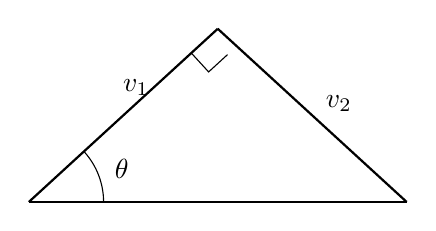
\begin{tikzpicture}[scale=1.0]
  \coordinate (O) at (0,0);
  \coordinate (P) at (2.4,2.2);
  \coordinate (Q) at (4.8,0);
  \draw[thick] (O) -- (P);
  \draw[thick] (P) -- (Q);
  \draw[thick] (O) -- (Q);
  \draw ($(P)!0.14!(O)$) -- ++(0.22,-0.24) -- ++(0.24,0.22);
  \draw (0.95,0) arc[start angle=0,end angle=42,radius=0.95];
  \node at (1.18,0.42) {$\theta$};
  \node[left] at (1.65,1.45) {$v_1$};
  \node[right] at (3.65,1.25) {$v_2$};
\end{tikzpicture}
\caption{Segitiga bantu untuk membaca sudut rotasi dari arah sumbu mayor.}
\label{fig:rotation-angle}
\end{figure}

Gambar~\ref{fig:rotation-angle} hanya berfungsi sebagai aid visual: arah sumbu mayor direpresentasikan oleh segitiga siku-siku sederhana, sehingga \(\theta\) langsung dapat dibaca dari perbandingan dua sisi yang ditandai. Dari rasio kedua sumbu tersebut juga diperoleh eksentrisitas \(e=0.7892\).

\begin{table}[h]
\centering
\caption{Karakteristik geometris elips hasil pemodelan lintasan bintang.}
\label{tab:star-geometry}
\begin{tabular}{ll}
\toprule
Parameter & Nilai \\
\midrule
Pusat $(x_0,y_0)$ & $(3.0343,\ 5.0700)$ \\
Semi-major axis $a$ & 4.9331 \\
Semi-minor axis $b$ & 3.0294 \\
Sudut rotasi $\theta$ & $43.19^\circ$ \\
Eksentrisitas $e$ & 0.7892 \\
Diskriminan $B^2-4AC$ & $-0.04773$ \\
\bottomrule
\end{tabular}
\end{table}

Tabel~\ref{tab:star-geometry} menegaskan bahwa koefisien aljabar yang diperoleh benar-benar memiliki arti geometris yang jelas. Elips hasil model tidak sejajar dengan sumbu koordinat, cukup lonjong, dan memiliki pusat yang bergeser dari titik asal. Dengan demikian, solusi least squares tidak hanya kecil residual-nya, tetapi juga menghasilkan bentuk kurva yang secara geometris masuk akal untuk mewakili lintasan orbit yang diamati.

\subsection{Validasi Visual}
Laporan sumber juga menyertakan dua visualisasi penting. Visualisasi pertama menumpangkan kurva elips hasil QR Householder di atas 300 titik observasi. Hasil overlay tersebut menunjukkan bahwa kurva mengikuti sebaran data dengan baik dan tidak menyisakan deviasi sistematis yang mencolok. Visualisasi kedua membandingkan kurva hasil Normal Equation dan QR Householder dalam satu bidang yang sama. Kedua kurva secara visual nyaris tidak dapat dibedakan, konsisten dengan fakta bahwa residual keduanya identik dan selisih parameter hanya muncul pada orde sangat kecil.

\begin{figure}[H]
\centering

\includegraphics[width=0.78\textwidth]{assets_nomor2/plot_ellipse_fit.png}
\caption{Overlay data observasi dengan elips hasil QR Householder.}
\label{fig:star-ellipse-fit}
\end{figure}

Gambar~\ref{fig:star-ellipse-fit} mendukung interpretasi bahwa model hasil QR Householder memang menangkap bentuk global lintasan dengan baik. Sumbu mayor, sumbu minor, dan pusat elips yang dihitung secara analitik juga konsisten dengan visualisasi ini.

\begin{figure}[H]
\centering

\includegraphics[width=0.78\textwidth]{assets_nomor2/plot_comparison.png}
\caption{Perbandingan visual kurva Normal Equation dan QR Householder.}
\label{fig:star-comparison}
\end{figure}

Gambar~\ref{fig:star-comparison} memperlihatkan bahwa kedua kurva praktis bertumpuk. Dengan kata lain, bila yang dilihat hanya hasil akhir pada data ini, keduanya memang tampak sama baik. Ini menjelaskan mengapa residual keduanya sama, sekaligus menegaskan bahwa alasan pemilihan QR bukan karena ia memberi fit yang secara visual jauh berbeda, melainkan karena ia mencapainya dengan stabilitas numerik yang lebih baik.

Dengan demikian, validasi visual mendukung dua kesimpulan numerik sekaligus. Pertama, model elips yang diperoleh memang cukup baik untuk menangkap pola lintasan bintang. Kedua, perbedaan antara dua metode bukan terletak pada kualitas fit akhir yang terlihat oleh mata, melainkan pada stabilitas cara solusi itu diperoleh.

\section{Kesimpulan}
Pemodelan lintasan bintang pada bagian ini memperlihatkan bagaimana persoalan geometri dapat ditangani secara sistematis melalui aljabar linear numerik. Dengan memodelkan 300 titik observasi sebagai sistem linear \emph{overdetermined}, dua metode least squares dapat dibandingkan secara langsung. Normal Equation dan QR Householder sama-sama menghasilkan koefisien elips yang nyaris identik serta residual error sebesar \(2.5082139462\).

Namun kesimpulan metodologisnya lebih tajam daripada itu. QR Householder tetap lebih layak dipilih karena bekerja dengan transformasi ortogonal dan tidak mengkuadratkan \emph{condition number}. Stabilitas inilah yang membuatnya lebih dapat diandalkan bila data menjadi lebih sensitif atau bila ukuran masalah diperbesar. Persamaan elips akhir yang diperoleh juga mempunyai interpretasi geometris yang jelas: pusat di sekitar \((3.0343, 5.0700)\), semi-major axis \(4.9331\), semi-minor axis \(3.0294\), sudut rotasi \(43.19^\circ\), dan eksentrisitas \(0.7892\). Dengan demikian, seperti pada laporan pertama, pilihan metode yang baik pada akhirnya tetap ditentukan oleh struktur numerik masalah, bukan hanya oleh bentuk solusi akhirnya.

\section*{Referensi Technical Report II}
\addcontentsline{toc}{section}{Referensi Technical Report II}
\begin{enumerate}[leftmargin=1.25em]
  \item Burden, R. L., dan Faires, J. D. (2011). \emph{Numerical Analysis}. Brooks/Cole.
  \item Golub, G. H., dan Van Loan, C. F. (2013). \emph{Matrix Computations}. Johns Hopkins University Press.
  \item Trefethen, L. N., dan Bau, D. (1997). \emph{Numerical Linear Algebra}. SIAM.
  \item Anton, H., dan Rorres, C. (2013). \emph{Elementary Linear Algebra: Applications Version}. Wiley.
  \item Stewart, J. (2015). \emph{Calculus: Early Transcendentals}. Cengage.
\end{enumerate}

\section*{Lampiran: Repositori dan Asal Berkas}
\addcontentsline{toc}{section}{Lampiran: Repositori dan Asal Berkas}
Seluruh kode yang relevan terhadap \emph{Technical Report I} tersedia pada repositori GitHub berikut:
\begin{center}
\url{https://github.com/dinovaslate/untitled1}
\end{center}

Berkas utama yang dipakai pada laporan pertama adalah sebagai berikut.
\begin{enumerate}[leftmargin=1.5em]
  \item \texttt{block\_lu\_cpu.py}, yang memuat implementasi Block LU pada CPU.
  \item \texttt{block\_lu\_gpu.py}, yang memuat implementasi Block LU pada GPU.
  \item \texttt{thomas\_algorithm.py}, yang memuat implementasi Thomas algorithm.
  \item \texttt{benchmark\_tridiagonal\_html.py}, yang digunakan untuk eksperimen perbandingan pada matriks tridiagonal.
\end{enumerate}

Untuk \emph{Technical Report II}, source program yang diberikan pengguna melalui archive nomor 2 sekarang juga tersedia dan artefak utamanya disalin ke folder \texttt{assets\_nomor2}. Berkas yang paling relevan adalah sebagai berikut.
\begin{enumerate}[leftmargin=1.5em]
  \item \texttt{pemodelan\_lintasan\_bintang.m}, yaitu script MATLAB utama untuk formulasi model, penyelesaian dengan Normal Equation dan QR Householder, analisis kompleksitas, serta ekstraksi parameter geometris elips.
  \item \texttt{data.csv}, yaitu data 300 titik observasi yang dipakai sebagai masukan.
  \item \texttt{plot\_ellipse\_fit.png} dan \texttt{plot\_comparison.png}, yaitu visualisasi hasil yang dipakai kembali pada bagian validasi visual laporan kedua.
\end{enumerate}

\end{document}
